\begin{figure}[htbp]
\centering
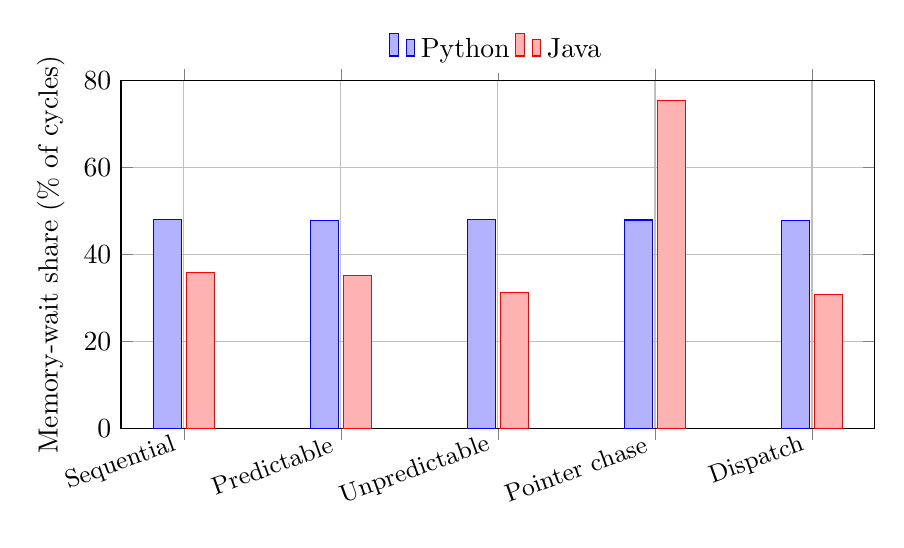
\begin{tikzpicture}
\begin{axis}[
  width=0.92\textwidth,
  height=6cm,
  ybar,
  bar width=10pt,
  symbolic x coords={Sequential,BranchPredictable,BranchUnpredictable,PointerChase,DynamicDispatch},
  xtick=data,
  xticklabels={Sequential,Predictable,Unpredictable,Pointer chase,Dispatch},
  x tick label style={rotate=20,anchor=east,font=\small},
  ylabel={Memory-wait share (\% of cycles)},
  ymin=0, ymax=80,
  ytick={0,20,40,60,80},
  grid=major,
  legend style={at={(0.5,1.02)},anchor=south,legend columns=2,draw=none},
]
\addplot coordinates {(Sequential,48.11) (BranchPredictable,47.89) (BranchUnpredictable,48.17) (PointerChase,47.96) (DynamicDispatch,47.75)};
\addplot coordinates {(Sequential,35.83) (BranchPredictable,35.29) (BranchUnpredictable,31.28) (PointerChase,75.46) (DynamicDispatch,30.93)};
\legend{Python,Java}
\end{axis}
\end{tikzpicture}
\caption{Memory-wait share by workload, using the simulator rule described in the text.}
\label{fig:memory-wait}
\end{figure}
